\section{Gaussian Processes}
\begin{frame}{Background}
    \begin{block}{Function Approximation}
        $\mathrm{f}:x \mapsto y$
    \end{block}
    \pause
    \begin{block}{Parametric Models: Pros}
        Easy to interpret
    \end{block}
    \begin{block}{Parametric Models: Cons}
        \begin{itemize}
            \item Simpler models lack expressive power
            \item Complex models require lots of data
            \item Predictions are dependent on the model
            \item Representation of uncertainty in the input space
            \end{itemize}
    \end{block}
\end{frame}

\begin{frame}{Linear Regression Model}
    $y = x+0.005x^2+ \epsilon$, $x \in [1,10] \cup [21,25]$,  $\epsilon \sim \mathcal{N}(0,10)$ 
    \begin{figure}
        \centering
        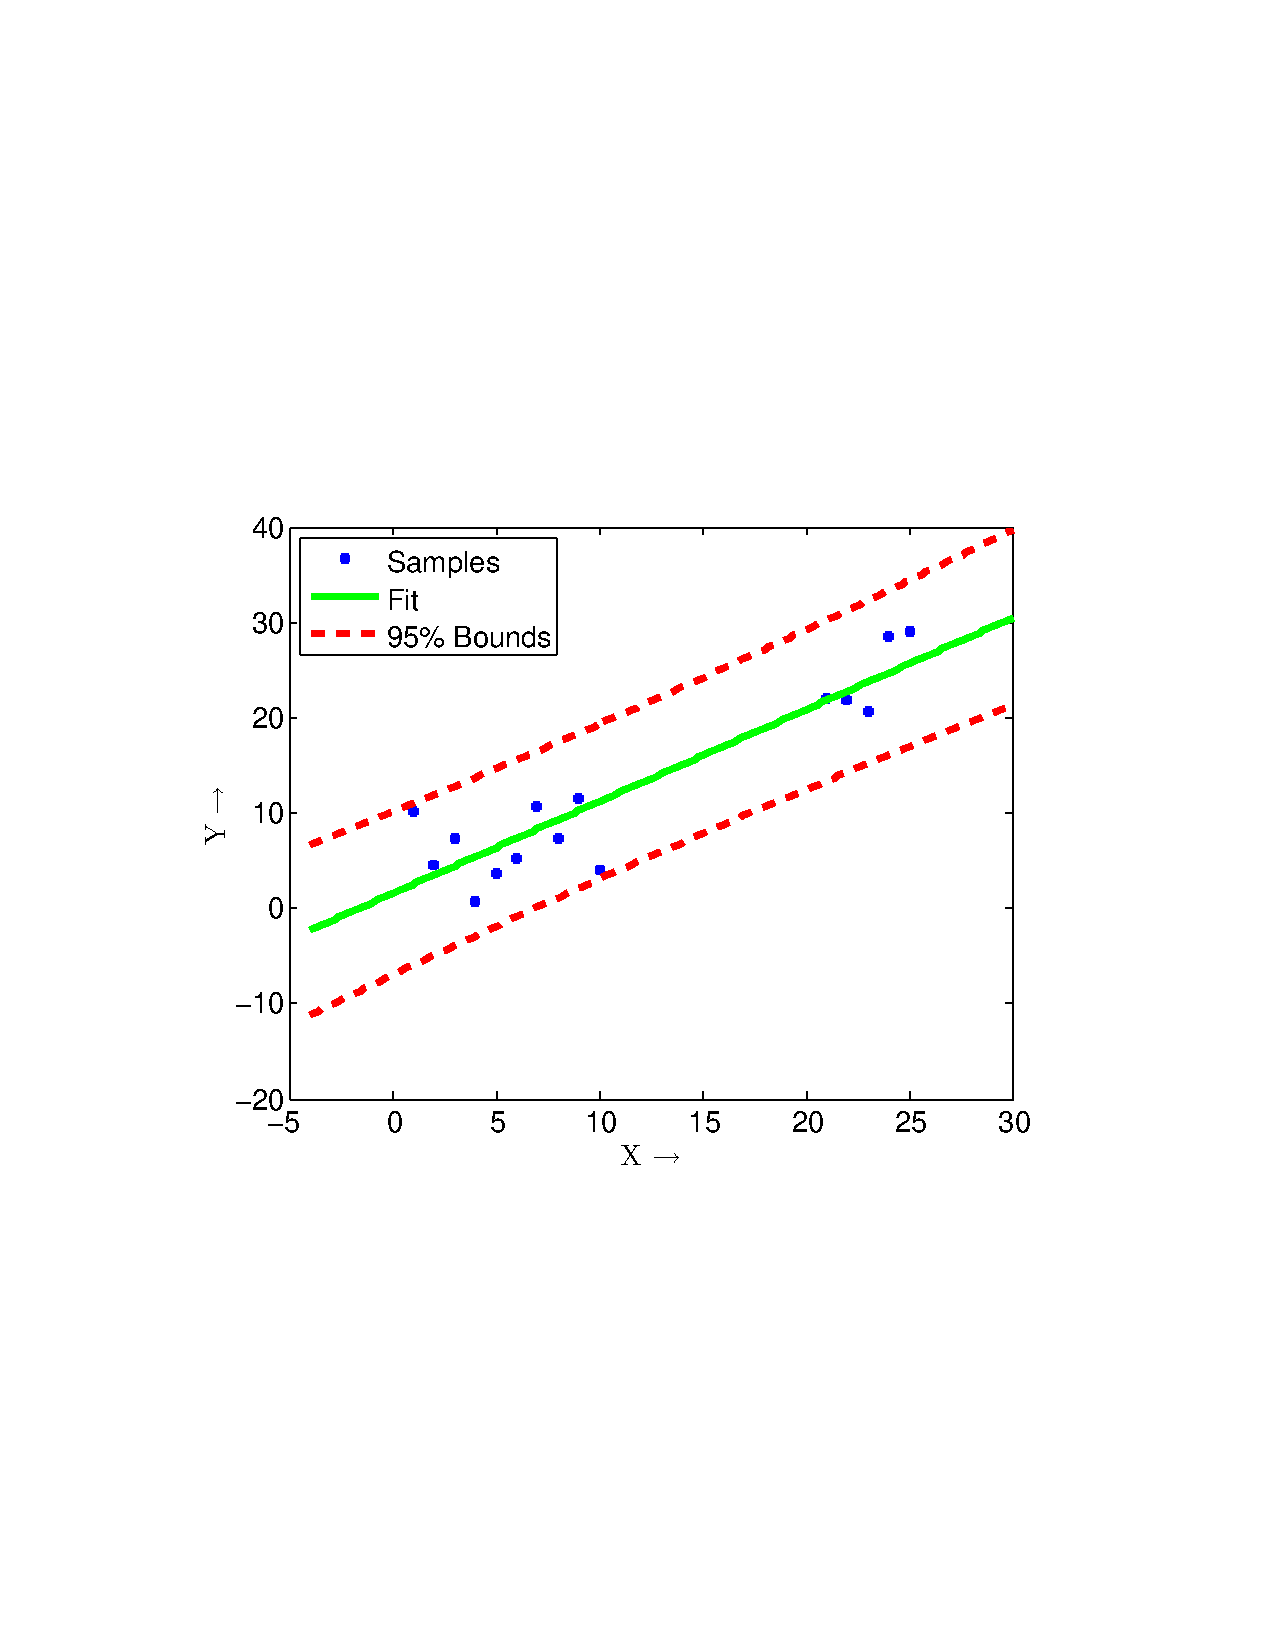
\includegraphics[width=0.5\linewidth,trim=30mm 80mm 40mm 70mm,clip]{figures/linear_fit}
        \caption{Linear Regression yields the model $y=mx+c$ with $m = 0.9644$ and $c = 1.5891$ }
    \end{figure}
\end{frame}

\begin{frame}{Quadratic Regression Model}
$y = x+0.005x^2+ \epsilon$, $x \in [1,10] \cup [21,25]$,  $\epsilon \sim \mathcal{N}(0,10)$
\begin{figure}
    \centering
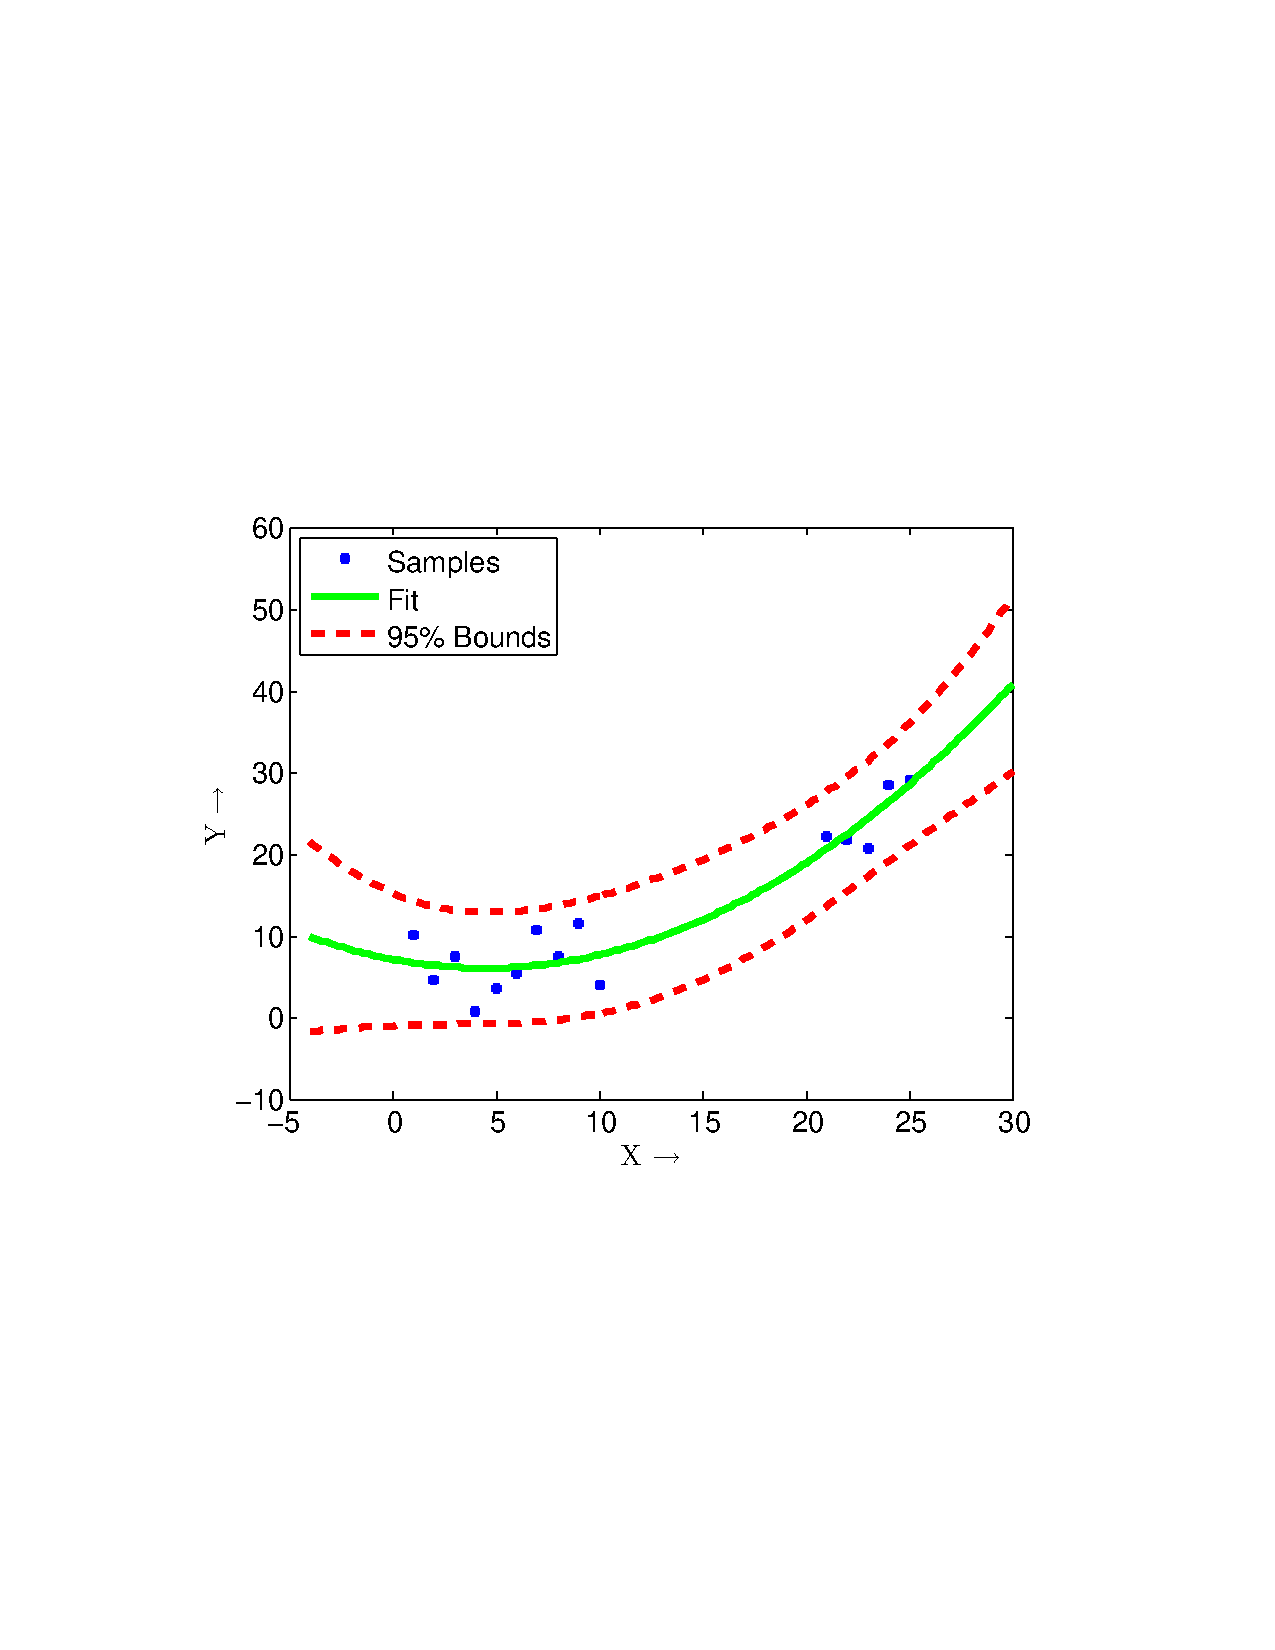
\includegraphics[width=0.5\linewidth,trim=30mm 80mm 40mm 70mm,clip]{figures/quadratic_fit}
\caption{ Quadratic model yields the model $y = ax^2+bx+c$ with $a = 0.0534$, $b = -0.04781$ and $c = 7.1231$}
\end{figure}

\end{frame}

\begin{frame}{Bayesian Linear Regression}
$y = x+0.005x^2+ \epsilon$, $x \in [1,10] \cup [21,25]$,  $\epsilon \sim \mathcal{N}(0,10)$ 
\begin{figure}
\centering
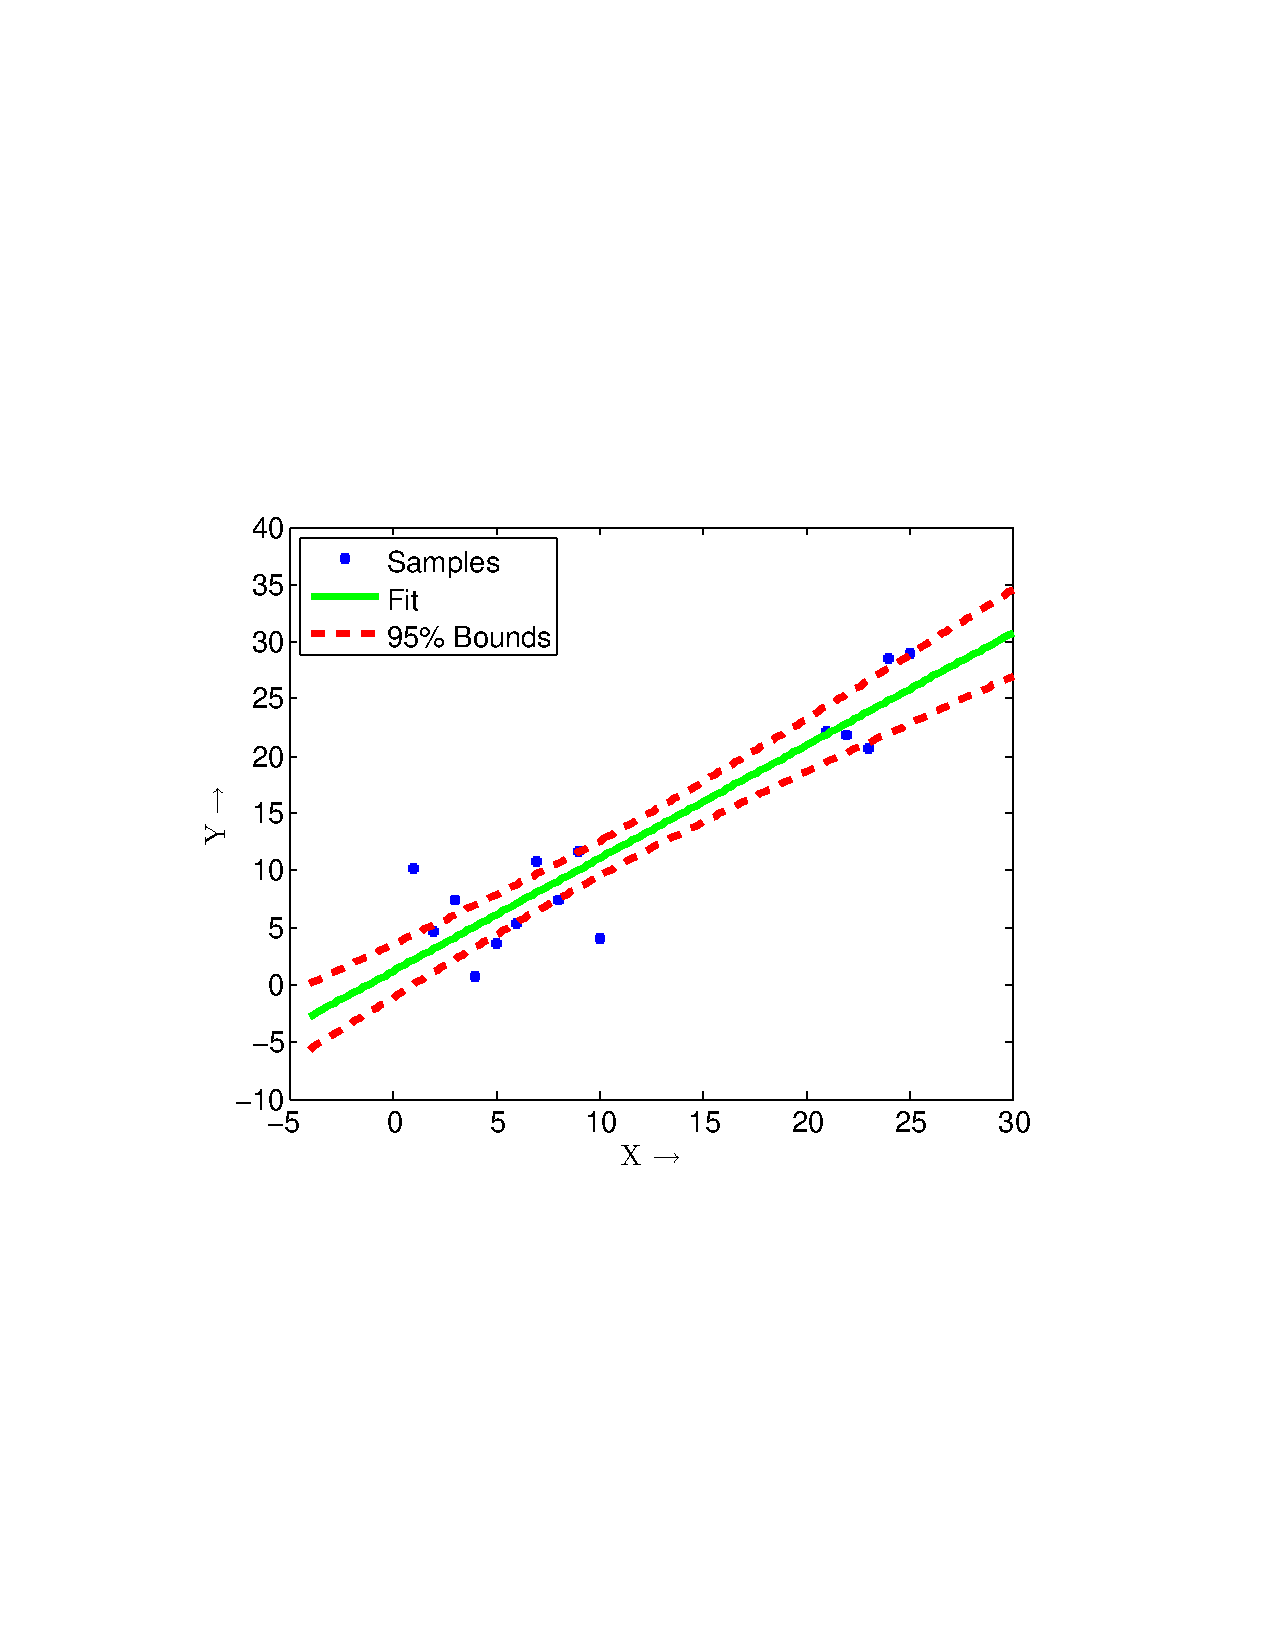
\includegraphics[width=0.5\linewidth,trim=30mm 80mm 40mm 70mm,clip]{figures/bayesian_linear_fit}
\caption{ Bayesian Regression fit uses a zero mean Gaussian observation noise with  variance $10$ and a zero mean Gaussian with diagonal variance $5$ prior on slope and intercept. The estimation process results in a mean parameter estimate of $0.9867$ slope and $1.1797$ intercept.}
\end{figure}
\end{frame}

\begin{frame}{Gaussian Process}
    \begin{block}
        Gaussian Process is a collection of random variables, any finite number
        of which are joint Gaussian distribution.
    \end{block}
    Non-parametric does not mean no parameters. Parametric models can through
    away data once parameters are tuned.
\end{frame}

\begin{frame}{Introduction}

\end{frame}

\begin{frame}{Introduction}

\end{frame}

\begin{frame}{Introduction}

\end{frame}

\begin{frame}{Introduction}

\end{frame}

\begin{frame}{Gaussian Process Regression}
$y = x+0.005x^2+ \epsilon$, $x \in [1,10] \cup [21,25]$,  $\epsilon \sim \mathcal{N}(0,10)$ 
\begin{figure}
\centering
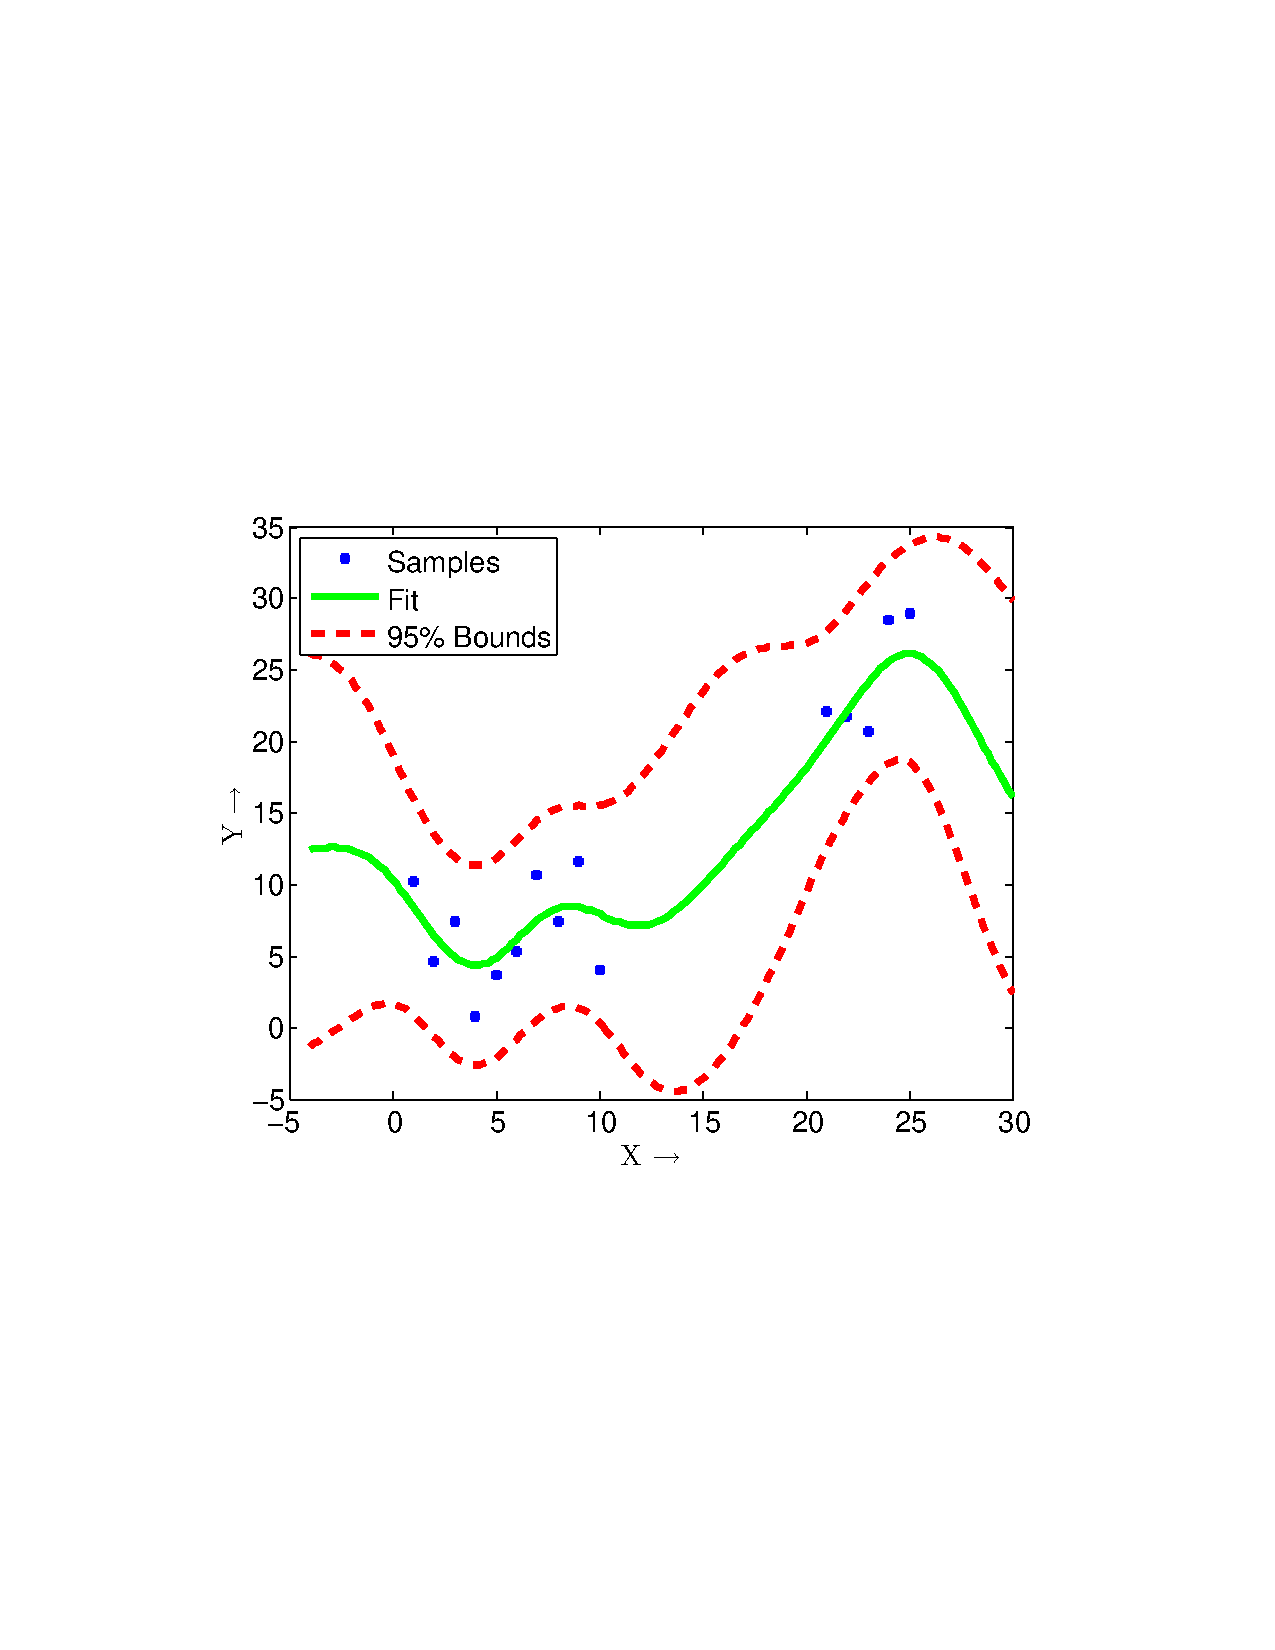
\includegraphics[width=0.5\linewidth,trim=30mm 80mm 40mm 70mm,clip]{figures/gpml_fit}
\caption{ GPR with constant mean function, Gaussian likelihood and Squared Exponential covariance function}
\end{figure}
\end{frame}


